\documentclass[letter,12pt]{article}
\usepackage[paperheight=27.94cm,paperwidth=21.59cm,bindingoffset=0in,left=3cm,right=2.0cm, top=3.5cm,bottom=2.5cm, headheight=200pt, headsep=1.0\baselineskip]{geometry}
\usepackage{graphicx,lastpage}
\usepackage{upgreek}
\usepackage{censor}
\usepackage[spanish,es-tabla]{babel}
\usepackage{pdfpages}
\usepackage{tabularx}
\usepackage{graphicx}
\usepackage{adjustbox}
\usepackage{xcolor}
\usepackage{colortbl}
\usepackage{rotating}
\usepackage{multirow}
\usepackage[utf8]{inputenc}
\usepackage{float}
\usepackage{hyperref}

\renewcommand{\tablename}{Tabla}
\usepackage{fancyhdr}
\pagestyle{fancy}


%
\begin{document}
%
   \title{\Huge{Informe Laboratorio 5}}

   \author{\textbf{Sección x} \\  \\Alumno x \\ e-mail: alumno.contacto@mail.udp.cl}
          
   \date{Junio de 2024}

   \maketitle

   \newpage
   
   \tableofcontents
 
  \newpage
  

\section*{Descripción de actividades}
\addcontentsline{toc}{section}{Descripción de actividades}
Para este último laboratorio, nuestro informante ya sabe que puede establecer un medio seguro sin un intercambio previo de una contraseña, gracias al protocolo diffie-hellman. El problema es que ahora no sabe si confiar en el equipo con el cual establezca comunicación, ya que las credenciales de usuario pueden haber sido divulgadas por algún soplón.\\

Para el presente laboratorio deberá:

\begin{itemize}
    \item Crear 4 contenedores en Docker o Podman, donde cada uno tendrá el siguiente SO:
        Ubuntu 16.10, Ubuntu 18.10, Ubuntu 20.10 y Ubuntu 22.10 a los cuales se llamarán C1, C2, C3 y C4 respectivamente.\\
        El equipo con Ubuntu 22.10 también será utilizado como S1.
        
    \item  Para cada uno de ellos, deberá instalar el cliente openSSH disponible en los repositorios de apt, y para el equipo S1 deberá también instalar el servidor openSSH.

    \item En S1 deberá crear el usuario \textquotedblleft\textbf{prueba}\textquotedblright con contraseña \textquotedblleft\textbf{prueba}\textquotedblright, para acceder a él desde los clientes por el protocolo SSH.
    
    \item En total serán 4 escenarios, donde cada uno corresponderá a los siguientes equipos:
    \begin{itemize}
        \item C1 $\rightarrow$ S1
        \item C2 $\rightarrow$ S1
        \item C3 $\rightarrow$ S1
        \item C4 $\rightarrow$ S1
    \end{itemize}
\end{itemize}

Pasos:

\begin{enumerate}
\item Para cada uno de los 4 escenarios, deberá capturar el tráfico generado por cada conexión con el server. A partir de cada handshake, deberá analizar el patrón de tráfico generado por cada cliente y adicionalmente obtener el HASSH que lo identifique. De esta forma podrá obtener una huella digital para cada cliente a partir de su tráfico. Cada HASSH deberá compararlo con la base de datos HASSH disponible en el módulo de TLS, e identificar si el hash obtenido corresponde a la misma versión de su cliente.\\\\
Indique el tamaño de los paquetes del flujo generados por el cliente y el contenido asociado a cada uno de ellos. Indique qué información distinta contiene el escenario siguiente (diff incremental). El objetivo de este paso es identificar claramente los cambios entre las distintas versiones de ssh.\\

\newpage

\item Para poder identificar que el usuario efectivamente es el informante, éste utilizará una versión única de cliente. ¿Con qué cliente SSH se habrá generado el siguiente tráfico?

\begin{figure}[ht]
    \centering
    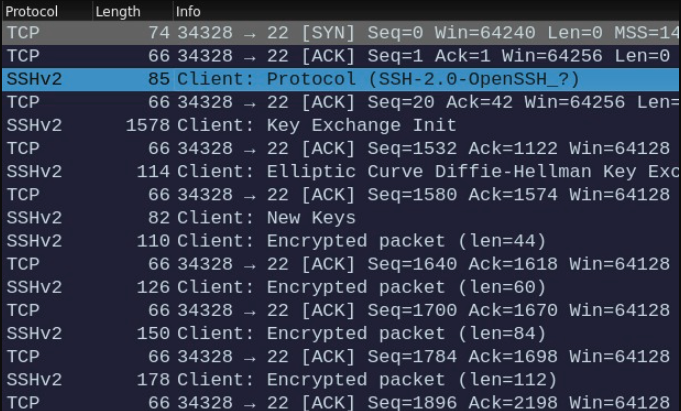
\includegraphics[width=1\linewidth]{Desarrollo/trafico.png}
    \caption{Tráfico generado del informante}
    \label{fig:trafico}
\end{figure}

Replique este tráfico generado en la imagen. Debe generar el tráfico con la misma versión resaltada en azul. Recuerde que toda la información generada es parte del sw, por lo tanto usted puede modificar toda la información.

\item Para que el informante esté seguro de nuestra identidad, nos pide que el patrón del tráfico de nuestro server también sea modificado, hasta que el Key Exchange Init del server sea menor a 300 bytes. Indique qué pasos realizó para lograr esto.

\begin{figure}[ht]
    \centering
    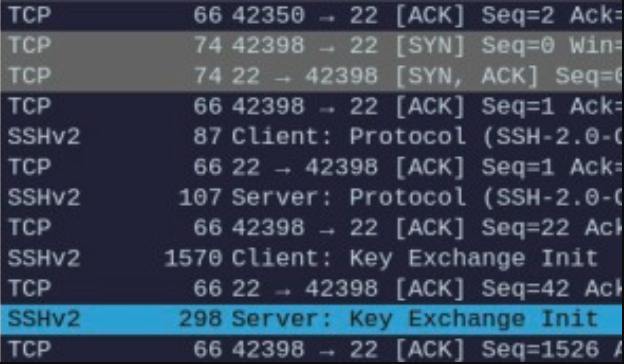
\includegraphics[width=1\linewidth]{Desarrollo/exchange.png}
    \caption{Captura del Key Exchange}
    \label{fig:exchange}
\end{figure}

\end{enumerate}

\section{Desarrollo (Parte 1)}

\subsection{Códigos de cada Dockerfile}
\subsubsection{C1}
\subsubsection{C2}
\subsubsection{C3}
\subsubsection{C4/S1}

\subsection{Creación de las credenciales para S1}

\subsection{Tráfico generado por C1, detallando tamaño paquetes del flujo y el HASSH respectivo (detallado)}

\subsection{Tráfico generado por C2, detallando tamaño paquetes del flujo y el HASSH respectivo (detallado)}

\subsection{Tráfico generado por C3, detallando tamaño paquetes del flujo y el HASSH respectivo (detallado)}

\subsection{Tráfico generado por C4 (iface lo), detallando tamaño paquetes del flujo y el HASSH respectivo (detallado)}

\subsection{Compara la versión de HASSH obtenida con la base de datos para validar si el cliente corresponde al mismo}

\subsection{Tipo de información contenida en cada uno de los paquetes generados en texto plano}
\subsubsection{C1}
\subsubsection{C2}
\subsubsection{C3}
\subsubsection{C4/S1}

\subsection{Diferencia entre C1 y C2}

\subsection{Diferencia entre C2 y C3}

\subsection{Diferencia entre C3 y C4}

\newpage

\section{Desarrollo (Parte 2)}

\subsection{Identificación del cliente SSH con versión \textquotedblleft?\textquotedblright}

\subsection{Replicación de tráfico al servidor (paso por paso)}

\section{Desarrollo (Parte 3)}

\subsection{Replicación del KEI con tamaño menor a 300 bytes (paso por paso)}

\section*{Conclusiones y comentarios}
\subsection*{Issues}
\end{document}
